\capitulo{4}{Técnicas y herramientas}

Aquí vamos a ver las tecnologías y herramientas más importantes que usamos para hacer este sistema, y por qué las elegimos para el proyecto. También explicaré cómo está montado todo en general y cómo se comunican las diferentes partes del sistema.

Diseñamos el sistema usando Blender, un programa de modelado 3D. Para programarlo, usamos Python y nos apoyamos mucho en la API 'bpy' de Blender, que nos ayuda a vigilar lo que pasa y a automatizar cosas. Juntas, estas herramientas nos permiten recoger, guardar y estudiar lo que hace el usuario mientras modela.

\section{Blender como entorno de desarrollo}

Elegimos Blender como nuestro programa principal de desarrollo porque nos deja acceder a la información de las escenas 3D desde código y es muy fácil de extender.

Una de las cosas buenas de Blender es que es software libre. Eso significa que podemos crear soluciones a medida sin los problemas que suelen tener los programas de pago. Además, tiene una API pública, con mucha documentación, que nos deja llegar a muchas cosas de dentro del programa, como objetos, geometrías, materiales, cámaras, luces o cómo se mueven las cosas en el espacio.

También es importante que podemos añadirle más funciones haciendo \textit{addons} (complementos) con Python. Así, podemos meter herramientas específicas justo donde el usuario las necesita, sin tocar el código principal de Blender. Esto hace que el sistema sea más flexible y fácil de organizar.

Y no menos importante es su gran comunidad de desarrolladores y la cantidad de documentación técnica que hay. Esto nos ayuda mucho para mantener el proyecto, hacerlo crecer si hace falta y solucionar cualquier problema que surja.

\section{Python como lenguaje de implementación}

Una vez que decidimos usar Blender, necesitábamos un lenguaje que pudiera integrarse bien con su API interna.

Para este proyecto usamos Python, ya que es el lenguaje oficial de Blender para crear scripts y desarrollar \textit{addons}.

Elegimos Python porque es fácil de leer, se integra muy bien con Blender y permite automatizar tareas y procesar datos de forma sencilla. Además, cuenta con muchas librerías útiles para análisis de información y generación de gráficos.

Gracias a esta integración, el sistema puede acceder al estado de la escena en tiempo real y registrar automáticamente las acciones que realiza el usuario mientras modela.

\section{API bpy}

Blender tiene algo que se llama 'bpy', que es como una interfaz de programación. Con ella, podemos meternos en los distintos componentes internos del programa de modelado usando código.

La API 'bpy' es la forma principal en que nuestro sistema se comunica con Blender. Nos permite ver y cambiar cosas de la escena activa al momento.

Para acceder a estos componentes, la API nos proporciona información sobre ellos: la escena, los objetos de la escena, las formas de las mallas, los materiales y texturas, las cámaras y las luces, la movilidad de los objetos en el espacio, las relaciones entre todos ellos, y algunas propiedades internas del programa.

No solo podemos conocer la estructura de la escena; la API nos permite llevar a cabo tareas automatizadas y estar siempre al tanto de los eventos dentro del programa.

Con todo esto, nuestro sistema puede detectar automáticamente muchas cosas que hace el usuario, como cuando crea o borra objetos, cambia de modo de edición, modifica puntos, líneas o caras, mueve cosas en el espacio o cambia la forma de las mallas.

Usar 'bpy' es clave para poder registrar y analizar datos sin tener que tocar cómo funciona Blender por dentro.

\section{Sistema de monitorización mediante handlers}

El sistema que creamos para recoger información funciona con  \textit{handlers} . Estos son como unos mecanismos internos de Blender que se activan cuando pasa algo.

Los  \textit{handlers}  nos permiten vigilar automáticamente los cambios en la escena y ejecutar funciones concretas cuando el usuario hace algo. Así, podemos tener un sistema que reacciona a los eventos, guardando información al momento sin molestar al usuario mientras modela.

Cada vez que el usuario hace algo en Blender, el sistema puede darse cuenta de los cambios importantes en la escena y empezar a analizar y guardar la información.

Nuestro sistema de vigilancia funciona detectando eventos sin parar mientras se está modelando. Cada vez que el usuario hace algo en Blender, los  \textit{handlers}  que hemos puesto en marcha detectan esos cambios importantes en la escena y, sin más, se ponen a recoger y guardar la información.

La Figura~\ref{fig:handlers_flow} muestra de forma resumida el funcionamiento de los \textit{handlers} dentro del sistema.

\begin{figure}[H]
\centering
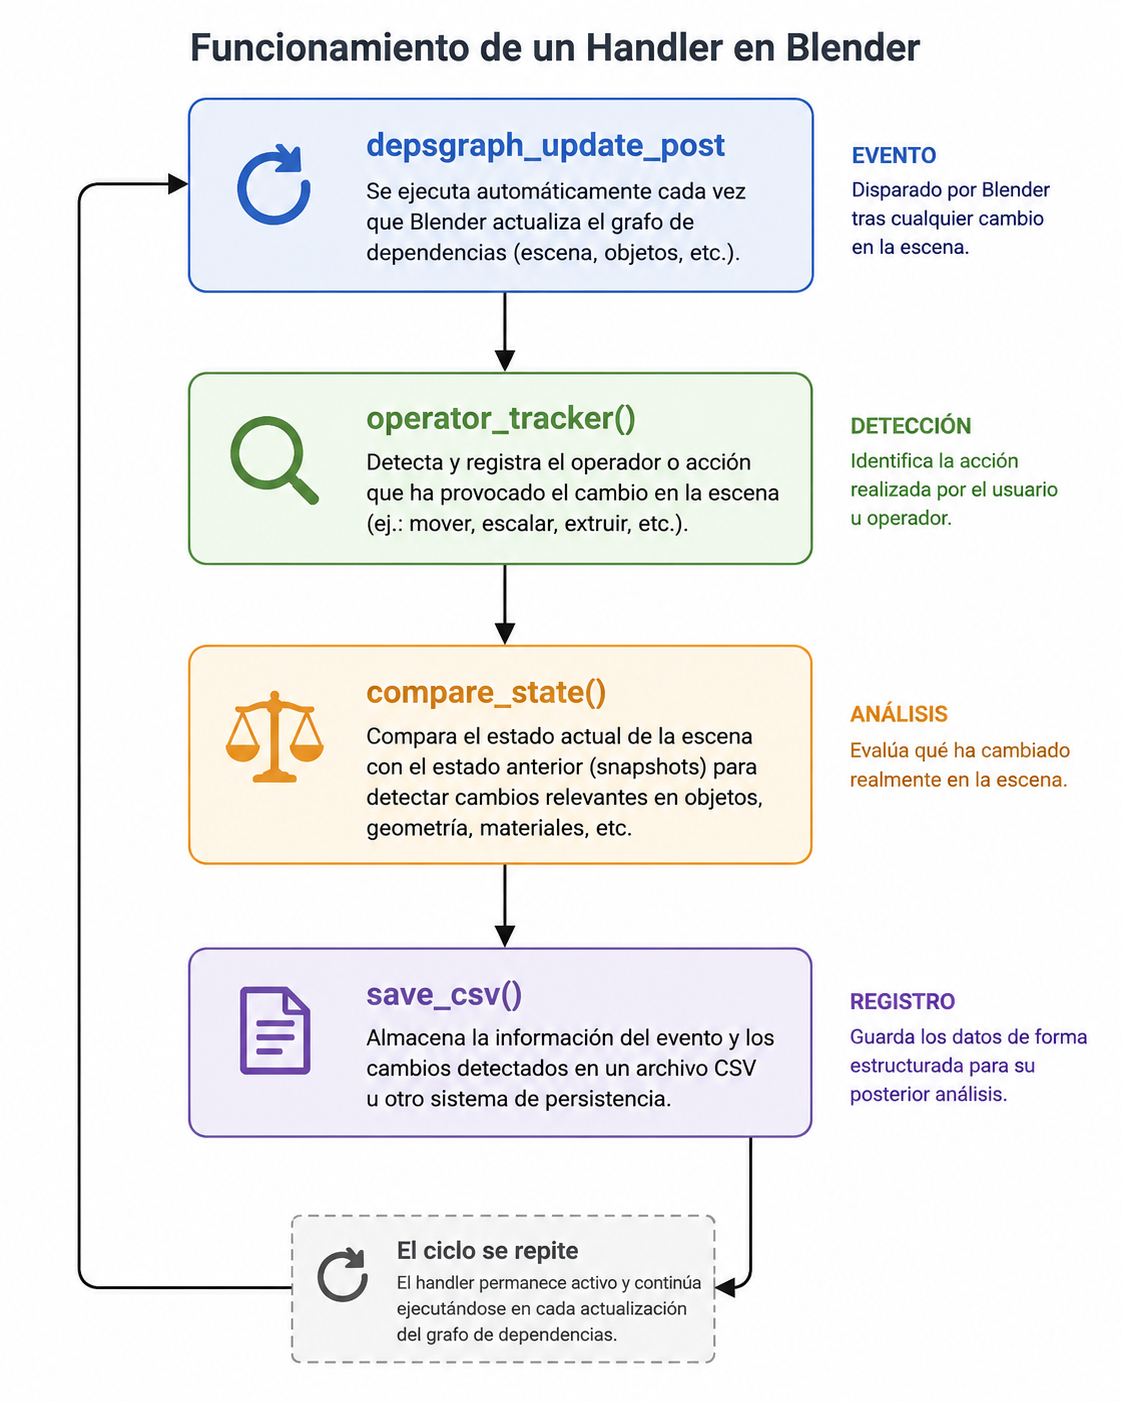
\includegraphics[width=0.75\textwidth]{diagramas/handler.png}
\caption{Proceso general de captura y almacenamiento de eventos dentro del sistema.}
\label{fig:handlers_flow}
\end{figure}

Gracias a esto, tenemos un sistema que vigila sin molestar, guardando información al momento sin interrumpir al usuario ni cambiar cómo funciona Blender por dentro.


\section{Persistencia de datos mediante archivos CSV}

Para guardar la información que recogemos durante el modelado, el sistema usa archivos CSV (del inglés 'valores separados por comas').

Elegimos este formato porque es muy simple de entender, no gasta muchos recursos y funciona muy bien con otros programas que usamos para analizar y procesar datos.

Los archivos CSV sirven para organizar la información en tablas, con filas y columnas. Así es más fácil tanto guardarla como procesar después los eventos que el sistema ha capturado.

Las principales ventajas de usar CSV son:

\begin{itemize}
\item es fácil de crear y exportar,
\item funciona con programas de estadística y análisis,
\item es sencillo de leer y procesar,
\item gasta pocos recursos,
\item y se integra sin problemas con otras aplicaciones.
\end{itemize}

Con esta forma de guardar los datos, podemos analizarlos más tarde, con otros procesos, sin que eso afecte al programa de modelado mientras se usa.


\section{Arquitectura del sistema}

El sistema está estructurado con un paradigma modular, alojado directamente dentro de Blender. Esta organizativa facilita la separación de las diversas responsabilidades del sistema, mejorando tanto la mantenibilidad como la expansión en el futuro.

El diálogo con Blender se efectúa mediante la interfaz programática \texttt{bpy}, que brinda acceso al código interno de los diversos componentes del entorno 3D, incluyendo escenas, objetos, geometría, transformaciones, materiales, o modos de edición.

A partir de esta API, el sistema utiliza distintos \textit{handlers} para monitorizar continuamente los cambios que ocurren mientras el usuario trabaja. Estos mecanismos funcionan como detectores de eventos que se ejecutan automáticamente cuando Blender actualiza la escena.

Gracias a este sistema de monitorización, el proyecto puede detectar acciones relacionadas con:

\begin{itemize}
    \item creación y eliminación de objetos,
    \item transformaciones espaciales,
    \item modificaciones geométricas,
    \item cambios de modo,
    \item operaciones sobre coordenadas UV,
    \item y uso de herramientas dentro del entorno de modelado.
\end{itemize}

Cuando se detecta un cambio relevante, la información pasa al \textit{addon} de captura de datos. Este módulo se encarga de analizar el evento, filtrar información innecesaria y organizar los datos registrados antes de almacenarlos.

El sistema de captura fue desarrollado siguiendo una estructura modular interna. Para ello, se separaron distintos componentes especializados en tareas concretas, como:

\begin{itemize}
    \item monitorización de eventos,
    \item análisis del estado de la escena,
    \item detección de operadores ejecutados,
    \item filtrado de cambios relevantes,
    \item y persistencia de datos.
\end{itemize}

Una vez procesada, la información se almacena en archivos CSV estructurados. Este formato permite mantener los registros organizados y facilita posteriormente el análisis externo de los datos generados durante las sesiones de modelado.

Después, el segundo \textit{addon} utiliza estos registros para realizar el análisis de métricas y generar representaciones visuales dentro del propio entorno de Blender.

El sistema de análisis también se organizó de forma modular. Internamente se divide en varios componentes responsables de:

\begin{itemize}
    \item lectura y procesamiento de archivos CSV,
    \item cálculo automático de métricas,
    \item generación de gráficos,
    \item representación tridimensional de datos,
    \item y visualización interactiva dentro de Blender.
\end{itemize}

Para generar las visualizaciones se combinaron librerías externas, como \textit{matplotlib}, junto con generación procedural de geometría dentro del espacio 3D de Blender. Gracias a esto, el sistema puede representar métricas mediante gráficos temporales, diagramas radar y visualizaciones espaciales directamente integradas en la escena.

La separación entre captura y análisis aporta varias ventajas importantes:

\begin{itemize}
    \item reduce el impacto sobre el rendimiento durante el modelado,
    \item facilita la organización interna del sistema,
    \item permite reutilizar los datos registrados posteriormente,
    \item y hace más sencilla la ampliación futura de nuevas métricas o representaciones visuales.
\end{itemize}

La Figura~\ref{fig:architecture_system} muestra la arquitectura general del sistema y el flujo principal de captura, almacenamiento y análisis de datos dentro de Blender.

\begin{figure}[H]
\centering
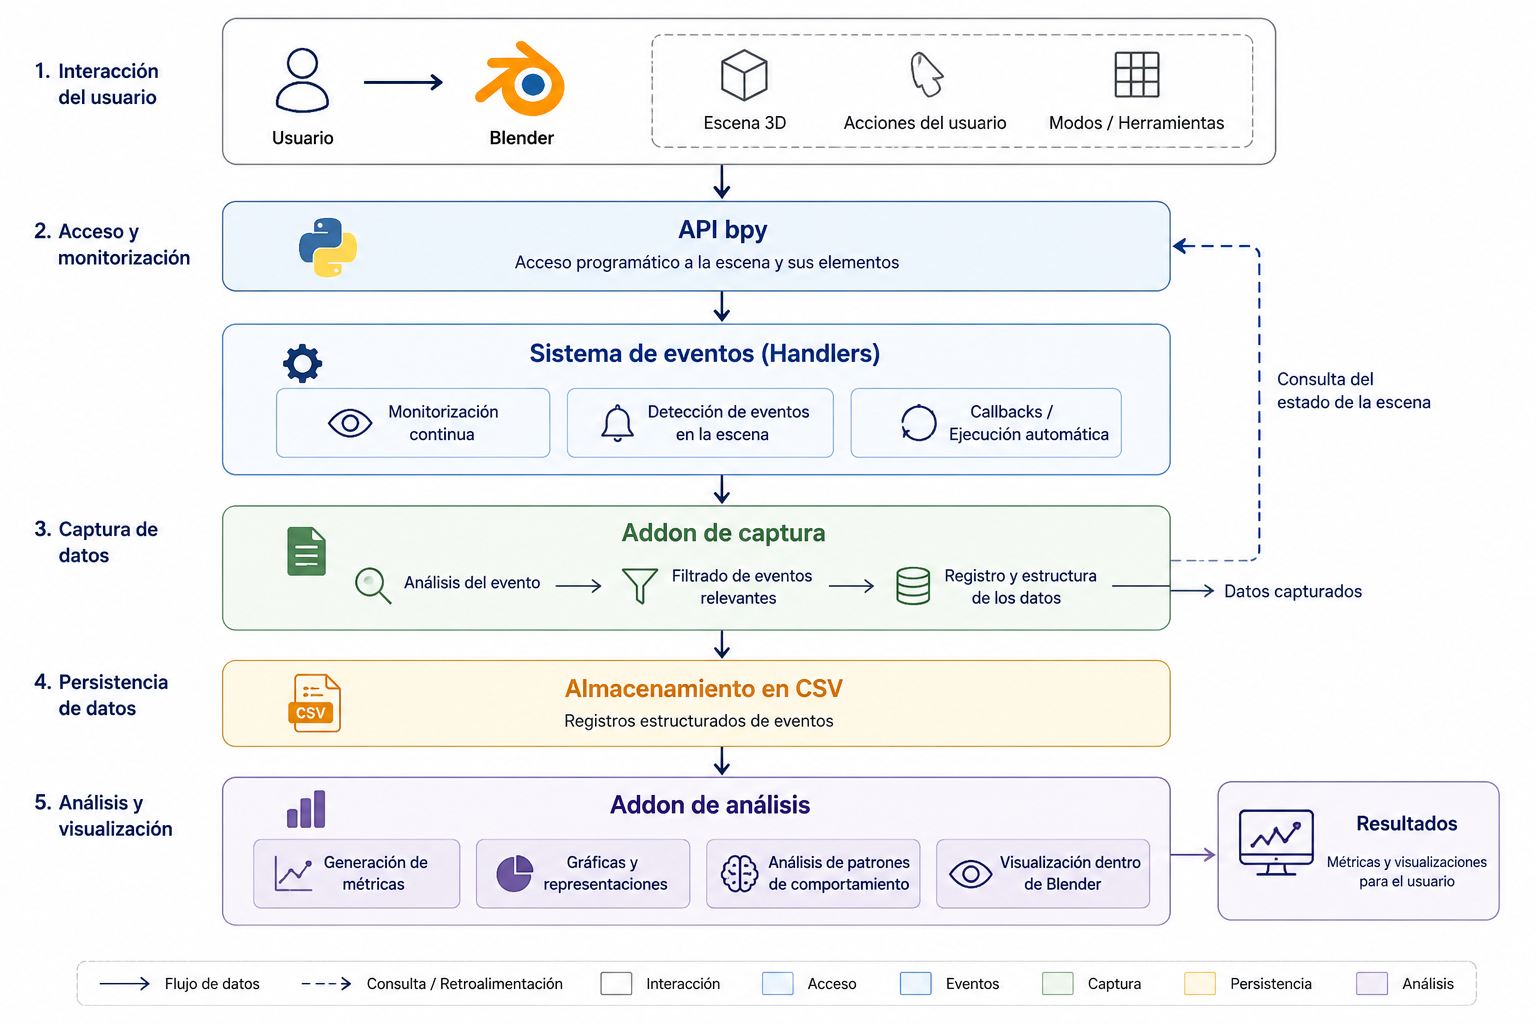
\includegraphics[width=0.95\textwidth]{diagramas/arquitecturaV2.png}
\caption{Arquitectura general del sistema desarrollado.}
\label{fig:architecture_system}
\end{figure}

\subsection{Addon de captura}

El 'addon' de captura es la parte que se encarga de vigilar todo el tiempo lo que hace el usuario dentro de Blender.

Este módulo funciona discretamente, por detrás, mientras el usuario modela. Usa los sistemas de vigilancia de Blender para encontrar los eventos importantes relacionados con lo que el usuario hace.

Sus funciones principales son:

\begin{itemize}
\item detectar qué pasa en la escena,
\item ver cómo está el programa de modelado,
\item identificar los cambios importantes,
\item guardar la información de esos eventos que detecta,
\item y almacenar los datos en archivos CSV.
\end{itemize}

Al diseñar este 'addon', queríamos que afectara lo mínimo posible al rendimiento general del sistema. Así, puede recoger información sin parar y de forma totalmente transparente para el usuario.

La Figura~\ref{fig:data_logger_sin_debug} muestra la interfaz del \textit{addon} de captura de datos.

\begin{figure}[H]
\centering
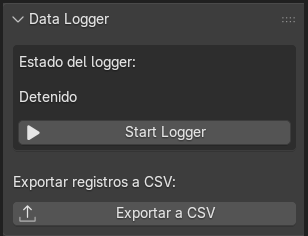
\includegraphics[
    width=0.8\textwidth,
    height=0.65\textheight,
    keepaspectratio
]{diagramas/data_logger_sin_debug.png}
\caption{Interfaz del \textit{addon} de captura de datos desarrollado para Blender.}
\label{fig:data_logger_sin_debug}
\end{figure}

\subsection{Addon de análisis}

El 'addon' de análisis usa la información que ya hemos guardado para crear métricas y gráficos que nos muestran cómo se ha comportado el usuario al modelar.

Este componente nos deja procesar los datos guardados y convertir esa información recogida en indicadores visuales y métricas fáciles de entender.

Sus funciones más importantes son:

\begin{itemize}
\item leer y procesar los datos,
\item crear métricas de forma automática,
\item hacer gráficos y representaciones visuales,
\item analizar cómo se comporta el usuario,
\item y mostrar los resultados directamente en Blender.
\end{itemize}

Con este 'addon', podemos ver de forma visual cómo avanza el modelado y entender cómo el usuario interactúa con la escena a lo largo del tiempo.

La Figura~\ref{fig:addon_analisis} muestra la interfaz del \textit{addon} de análisis.

\begin{figure}[H]
    \centering
    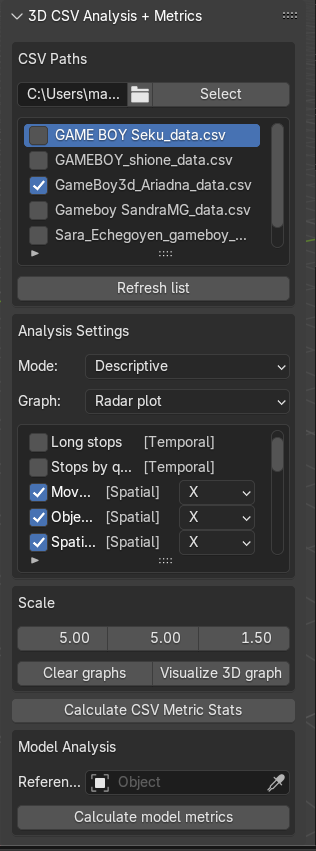
\includegraphics[width=0.4\textwidth]{diagramas/capture_addon_panel.png}
    \caption{Panel principal del addon de captura de datos dentro de Blender.}
    \label{fig:addon_analisis}
\end{figure}

\subsection{Estructura interna del addon de análisis}

El addon de análisis se organizó en distintos módulos independientes para separar las responsabilidades principales del sistema.

Algunos de los módulos más importantes son:

\begin{itemize}
    \item \texttt{metrics\_ui.py}: controla la interfaz principal y la interacción con el usuario.
    
    \item \texttt{graphs.py}: genera las representaciones visuales y geometría utilizada para visualizar métricas dentro de Blender.
    
    \item \texttt{utils.py}: contiene funciones auxiliares relacionadas con el cálculo y procesamiento de métricas.
    
    \item \texttt{\_\_init\_\_.py}: registra el addon y conecta los distintos componentes internos del sistema.
\end{itemize}

Este enfoque modular simplifica el mantenimiento del código y facilita el desarrollo de nuevas funciones sin necesidad de alterar los otros componentes del sistema.